\documentclass[10pt]{article}

\usepackage[margin=1in]{geometry}
\usepackage{mathptmx}
\usepackage{amsmath,amssymb}
\usepackage{booktabs}
\usepackage{tikz}
\usepackage{caption}
\usepackage{microtype}
\usepackage[hidelinks]{hyperref}
\usepackage{array}
\usepackage{ragged2e}

\captionsetup{font=small,labelfont=bf}
\setlength{\parskip}{0pt}
\setlength{\emergencystretch}{1.5em}

\title{\bfseries Beyond Token Count: Characterizing the Marginal Utility of Parallel Sampling, Tree Search, and Self-Consistency as Independent Axes of Inference Compute}
\author{Prateek Dutta\\ \small Industrial AI Researcher, India}
\date{}

\begin{document}

\maketitle

\begin{abstract}
\noindent Test-time compute has displaced pretraining scale as the dominant lever for improving large language model (LLM) reasoning, yet the literature routinely collapses heterogeneous inference strategies into a single ``more compute'' narrative. This review argues that parallel sampling with verifier selection, tree- and graph-structured search, and self-consistency-style answer aggregation constitute three distinct axes of inference compute, each governed by a different accuracy driver, cost model, and failure regime. Synthesizing results from more than forty studies published primarily between 2023 and 2026, the paper shows that reported scaling curves are not comparable across axes: cost accounting is inconsistent (samples, nodes, tokens, FLOPs, dollars), verifier quality is rarely isolated as a confound, and controlled single-axis ablations are almost absent. The review contributes a three-axis taxonomy, a cross-axis comparison of cost models and failure modes, and an open-problems agenda culminating in a concrete factorial experimental design for measuring the marginal utility of each axis under matched budgets. The central takeaway is that scaling behavior differs meaningfully across axes and task types, and that the field's aggregate ``accuracy versus compute'' curves obscure precisely the mechanisms they are meant to reveal.

\medskip
\noindent\textbf{Keywords---}test-time compute scaling; inference-time compute; parallel sampling; best-of-$n$; tree search; Monte Carlo tree search; self-consistency; majority voting; process reward models; large language model reasoning
\end{abstract}

\section{Introduction}
\label{sec:intro}

For half a decade, progress in language modeling was organized around training-compute scaling laws. Kaplan et al.\ established that loss falls predictably as a power law in parameters, data, and compute [1], and Hoffmann et al.\ corrected the allocation rule, showing that a 70B-parameter model trained on twenty tokens per parameter outperforms much larger undertrained models [2]. Subsequent analyses observed that this ``Chinchilla-optimal'' accounting ignores deployment: once inference demand is priced in, smaller models trained longer become preferable [3]. The release of OpenAI's o1 series marked a public inflection point, with the developers reporting that accuracy on competition mathematics improves smoothly with the amount of computation expended at answer time, not only with training scale [4,5]. DeepSeek-R1 reproduced this behavior in an open model trained by reinforcement learning, reaching 79.8\% pass@1 on AIME~2024 [6]. Test-time compute is now widely treated as the field's primary scaling lever.

This shift, however, has imported a conceptual sloppiness that the training-compute era largely avoided. Training FLOPs are a single, well-defined quantity; ``test-time compute'' is not. A model can spend inference computation in structurally different ways: by drawing more independent samples and selecting among them, by exploring a tree of partial solutions under the guidance of a value function, or by aggregating the final answers of many samples through voting. Most empirical papers nonetheless report one curve---pass@$k$, or accuracy against a loosely defined budget---without isolating which mechanism produced the gain. When Snell et al.\ report that compute-optimal test-time scaling outperforms a best-of-$N$ baseline by more than a factor of four [7], the improvement mixes search structure, verifier quality, and adaptive allocation; when Brown et al.\ report log-linear coverage growth across four orders of magnitude of samples [8], the curve says nothing about whether a selector can realize that coverage. The three mechanisms have different marginal-utility profiles, different parallelism characteristics, and different dependencies on auxiliary models, yet they are routinely aggregated under one label.

This paper is a critical literature review, not primary empirical work. Its contribution is threefold: (i) a taxonomy that treats parallel sampling, tree/graph search, and self-consistency as partially overlapping but analytically separable axes of inference compute; (ii) a synthesis of reported scaling results from 2023--2026 restated in a common vocabulary, with explicit attention to the inconsistent cost accounting that makes cross-paper comparison unreliable; and (iii) an open-problems agenda that specifies the controlled experiments the literature currently lacks, including a concrete factorial design intended as the basis for a follow-on empirical study. Welleck et al.\ provide the closest prior synthesis, organizing inference algorithms as ``meta-generators'' [9]; the present review differs by focusing narrowly on marginal utility per unit cost across axes and on the measurement failures that prevent the field from estimating it.

The remainder of the paper proceeds as follows. Section~\ref{sec:background} formalizes the three axes and fixes a shared cost unit. Section~\ref{sec:synthesis} reviews each axis in turn: foundational formalizations, reported scaling behavior, task affinities, and known limitations. Section~\ref{sec:comparison} compares the axes directly, via a structured table and a conceptual three-axis framework, and examines the sparse literature on axis combinations. Section~\ref{sec:open} develops the open-problems agenda and the proposed experimental design. Section~\ref{sec:conclusion} concludes.

\section{Background and Definitions}
\label{sec:background}

Let $p_\theta(y \mid x)$ denote an autoregressive LLM producing a response $y$ (possibly containing a reasoning trace) to prompt $x$, and let $\mathrm{ans}(y)$ extract a final answer. Chain-of-thought (CoT) prompting, which conditions the model to emit intermediate reasoning before its answer, is the substrate on which all three axes operate [10]. The axes are defined as follows.

\textbf{Axis 1: Parallel sampling with selection (best-of-$n$).} Draw $n$ independent samples $y_1,\dots,y_n \sim p_\theta(\cdot \mid x)$ at positive temperature and return $y^\ast = \arg\max_{i \le n} r(x, y_i)$, where $r$ is an external scoring function---a learned reward model, a trained verifier, or an exact checker such as unit tests or a proof assistant [11,12]. The samples are exchangeable and the compute is embarrassingly parallel. The ceiling of this axis is \emph{coverage}, defined by Brown et al.\ as ``the fraction of problems that are solved by any generated sample'' [8]; in code settings coverage coincides with the pass@$k$ metric formalized by Chen et al.\ [13]. Realized accuracy is coverage filtered through the precision of $r$.

\textbf{Axis 2: Tree and graph search.} Decompose generation into steps, maintain a frontier of partial solutions (tree nodes), score intermediate states with a value estimate $V(x, y_{1:t})$, and allocate expansion budget preferentially to promising states. Instantiations include Tree-of-Thoughts (ToT) with breadth-first or depth-first exploration and model self-evaluation [14], Monte Carlo tree search (MCTS) over reasoning steps [15,16], step-level beam search [17], and graph-structured generalizations that permit merging and refinement of partial thoughts [18]. The defining property is \emph{intermediate-state evaluation}: compute is redirected during generation, so the samples are no longer independent and the procedure is partially sequential.

\textbf{Axis 3: Self-consistency and answer-level aggregation.} Draw $k$ independent CoT samples and return the plurality answer, $y^\ast = \arg\max_a \sum_{i=1}^{k} \mathbf{1}[\mathrm{ans}(y_i) = a]$, marginalizing over reasoning paths rather than selecting a single trajectory [19]. No external scorer and no search structure are involved; the mechanism is purely statistical, exploiting the assumption that correct answers concentrate while errors disperse. Extensions replace exact answer matching with model-judged equivalence for free-form outputs [20] and with verifier-weighted votes [21].

Axes 1 and 3 share the sampling step and differ in the selection operator (learned scorer versus mode of the answer distribution); axis 2 differs from both in \emph{when} evaluation occurs (during rather than after generation). The three are therefore partially overlapping but not reducible to one another, and hybrid methods occupy the interior of the space (Section~\ref{sec:comparison}).

\textbf{Cost accounting.} Throughout, this review adopts \emph{total generated tokens per query} as the primary cost unit, converting to FLOPs where necessary via the standard approximation of roughly $2N_{\text{params}}$ FLOPs per generated token [1]. This choice is itself a finding of the review: the surveyed papers variously report sample count [19], node or LLM-call count [14], FLOPs [7,22], dollar cost [8,14], and wall-clock latency, and these units do not interconvert without assumptions the papers rarely state. Token count ignores parallelism---under batched serving, $n$ parallel samples cost approximately the latency of one, whereas a deep search tree or a long sequential reasoning chain cannot be parallelized across its own depth. Speculative decoding further decouples token count from latency by accepting multiple draft tokens per target-model step without changing the output distribution [23,24], so latency-based and token-based comparisons of inference strategies can order methods differently. Any cross-axis comparison must therefore state whether the budget is tokens, FLOPs, latency under fixed parallelism, or dollars; Section~\ref{sec:open} returns to this as an open problem.

\section{Literature Synthesis by Axis}
\label{sec:synthesis}

\subsection{Axis 1: Parallel Sampling with Verifier Selection}
\label{sec:axis1}

\textbf{Formalization.} Best-of-$n$ selection predates the reasoning literature: Stiennon et al.\ used reward-model reranking of summaries as a strong baseline for reinforcement learning from human feedback [25], and Nakano et al.\ found that best-of-$n$ against a reward model rivaled policy optimization for long-form question answering [26]. Cobbe et al.\ transplanted the recipe to mathematical reasoning, training a verifier on correctness labels and reporting that a 6B model with best-of-100 verification matched the gains of an approximately thirtyfold increase in model size on GSM8K [11]. The modern formal object is the best-of-$n$ policy itself, whose divergence from the base model Beirami et al.\ characterized analytically, showing that the commonly used $\log n - (n-1)/n$ KL formula is an upper bound that can be loose [27].

\textbf{Scaling behavior.} The clearest scaling evidence comes from Brown et al., who repeated sampling across four orders of magnitude and found that coverage grows approximately log-linearly, well modeled by an exponentiated power law in $n$ [8]. Where an exact verifier exists, the coverage curve is realized directly: on SWE-bench Lite, solved issues rose from 15.9\% at one sample to 56\% at 250 samples for DeepSeek-Coder-V2, and five samples of the cheaper model were more cost-effective at current API prices than a single sample from a frontier model [8]. OpenAI's o1 exhibits the same structure at the frontier: 74.4\% single-sample accuracy on AIME~2024 rising to 93\% when 1{,}000 samples are reranked by a learned scoring function [4]. With learned verifiers the picture is more qualified. Lightman et al.\ found that a process reward model (PRM) sustained best-of-$N$ gains to $N{=}1860$, solving 78.2\% of a MATH subset against 72.4\% for an outcome reward model, with the gap widening as $N$ grew [12]; process supervision had earlier been shown to reduce reasoning errors at matched final-answer accuracy [28]. Cheaper, automated step-label pipelines have narrowed the data-cost objection to PRMs [29,45].

\textbf{Task affinity.} The axis is strongest wherever candidate verification is cheaper or more reliable than candidate generation: competitive programming and software engineering with executable tests, formal proof with a proof checker [8,13], and mathematics with strong PRMs [12]. It transfers poorly to open-ended generation, where no exact checker exists and reward models must carry the full selection burden [25].

\textbf{Limitations.} Cost grows linearly in $n$ while accuracy grows roughly logarithmically at best, so marginal utility decays by construction [8]. More fundamentally, the axis inherits the defects of its selector. Gao et al.\ showed that as best-of-$n$ optimizes harder against a proxy reward model, gold-standard quality peaks and then declines---overoptimization occurs without any parameter updates [30]. Stroebl et al.\ formalized the consequence for resampling: with an imperfect verifier, false positives accumulate as $n$ grows, true accuracy can fall with additional compute, and weaker models suffer earlier because their generation and verification abilities are coupled [31]. Verifier precision, not sample budget, is thus the binding constraint on this axis.

\subsection{Axis 2: Tree and Graph Search}
\label{sec:axis2}

\textbf{Formalization.} Yao et al.\ introduced ToT, casting reasoning as search over ``thoughts''---coherent intermediate steps---with the model itself proposing successors and evaluating states, combined with classical breadth-first or depth-first control [14]. Hao et al.\ recast the LLM as a world model and applied MCTS over reasoning states [15]; Feng et al.\ showed that AlphaZero-style tree search with a learned value function can guide both decoding and subsequent training [16]. Xie et al.\ integrated self-evaluation into stochastic beam search at the step level [17]; Besta et al.\ generalized the tree to an arbitrary graph, permitting aggregation and refinement of partial solutions [18]. Value-guided decoding has also been applied outside mathematics, reusing the value network of a PPO-trained policy to steer token-level MCTS [32], and tree search has been lifted to agentic settings that interleave acting and planning [33].

\textbf{Scaling behavior.} The headline result remains ToT on Game of 24: GPT-4 with CoT solved 4\% of instances, best-of-100 CoT reached 49\%, and ToT with breadth five reached 74\% [14]---a gain that one hundred independent samples could not buy, illustrating that structure is not reducible to sample count. The paper's own cost analysis, however, shows ToT consuming roughly 5.5k generated tokens per case, about \$0.74 versus \$0.47 for best-of-100 CoT [14], and the tasks were selected because they require lookahead. On mathematics benchmarks the compute-matched evidence is more sobering. Wu et al.\ found that standard MCTS was dominated by simpler sampling strategies at equal FLOPs, because expanded-but-unused subtrees waste budget; their reward-balanced search (REBASE), which allocates expansion by softmax-weighted PRM scores, was Pareto-optimal, letting Llemma-7B match Llemma-34B accuracy on MATH at roughly half the FLOPs [22]. Snell et al.\ similarly found that PRM-guided step-level search outperforms best-of-$N$ mainly on harder prompts and at lower budgets, while plain sampling catches up on easier prompts as budget grows; exploiting this difficulty dependence adaptively yielded their headline fourfold efficiency gain and FLOPs-matched wins over models fourteen times larger [7]. Liu et al.\ extended the compute-optimal analysis across policy models, PRMs, and difficulty bins, reporting that with the right configuration a 1B model can exceed a 405B model on MATH-500---and that the best strategy is not stable across configurations [34]. Search integrated with self-improvement loops has pushed small-model mathematics furthest: MCTS-driven self-evolution with a process preference model raised a 7B model to approximately 90\% on MATH [35], with related designs in AlphaLLM, ReST-MCTS*, and mutual-consistency search over small models [36,37,38].

\textbf{Task affinity.} Search pays where the solution decomposes into steps whose partial correctness is estimable---puzzle-like planning [14], competition mathematics [22,35], and agentic tasks with environment feedback [33]. It underperforms per unit compute on tasks where the first step reveals little [7,22].

\textbf{Limitations.} The axis is hostage to its value estimate. Self-evaluation is noisy, and learned PRMs embed their own biases: Monte-Carlo-labeled PRMs misidentify step correctness often enough that naive training underperforms [29,39], and Setlur et al.\ argue that effective process rewards should measure \emph{progress} (step-level advantage) rather than absolute correctness, reporting substantially better search efficiency when they do [40]. Search also adds serial depth: node expansions depend on parent evaluations, so latency scales with tree depth in a way batched parallel sampling avoids (Section~\ref{sec:background}). Finally, search overhead is pure loss on instances the base policy already solves---the difficulty dependence documented by Snell et al.\ [7].

\subsection{Axis 3: Self-Consistency and Majority Voting}
\label{sec:axis3}

\textbf{Formalization.} Wang et al.\ introduced self-consistency as a replacement for greedy CoT decoding: sample diverse reasoning paths, then marginalize out the paths by plurality vote over final answers [19]. The method assumes a discrete, canonicalizable answer space; universal self-consistency relaxes this by having the model select the most consistent of its own free-form outputs [20], and DiVeRSe replaces uniform votes with verifier-weighted votes [21]. Adaptive-consistency makes the sample count dynamic, halting when the running plurality is statistically stable and cutting samples several-fold at negligible accuracy cost [41].

\textbf{Scaling behavior.} The original paper reported absolute gains over greedy CoT of +17.9\% on GSM8K, +11.0\% on SVAMP, +12.2\% on AQuA, +6.4\% on StrategyQA, and +3.9\% on ARC-challenge with roughly forty sampled paths, with most of the benefit realized well before that budget [19]. Saturation is the axis's signature: Brown et al.\ found majority voting plateaus beyond roughly one hundred samples even as coverage keeps climbing, leaving an expanding gap between what sampling finds and what voting can extract [8]. At the frontier the same shape recurs at smaller magnitudes: o1 gains about nine points from cons@64 on AIME (74.4\% to 83.3\%) but essentially nothing on GPQA Diamond (77.3\% to 78.0\%) [4,5], while DeepSeek-R1-Zero gains fifteen points on AIME (71.0\% to 86.7\%) [6]---the marginal value of voting depends jointly on task and on how peaked the model's answer distribution already is. Chen et al.\ supplied the sharpest caveat: accuracy as a function of the number of aggregated calls can be non-monotonic, because voting amplifies the modal answer, which on hard queries is wrong; the optimal $k$ depends on the difficulty mix of the workload [42].

\textbf{Task affinity.} Voting excels on tasks with short, exactly comparable answers and error diversity---arithmetic word problems, multiple choice, commonsense QA [19]. It degrades on tasks with large plausible-but-wrong answer mass [42], and it is inapplicable without modification to open-ended generation [20].

\textbf{Limitations.} Self-consistency cannot exceed the probability that the correct answer is modal; it converges to that ceiling and stops [8,42]. It discards all information in the reasoning paths except the final answer, which is precisely the information PRMs exploit---Lightman et al.\ found majority voting at $N{=}1860$ reached only 69.6\% where a PRM reached 78.2\% [12]. Its costs are often understated: like best-of-$n$ it multiplies token cost linearly, and unlike best-of-$n$ it cannot benefit from a better selector without ceasing to be self-consistency.

\section{Cross-Axis Comparison}
\label{sec:comparison}

Table~\ref{tab:axes} condenses the synthesis into a directly comparable form. Two structural observations follow.

\begin{table}[t]
\centering
\caption{The three axes of inference compute compared. $n,k$: number of samples; $L$: tokens per sample; $M$: nodes expanded; $\ell$: tokens per step; $d$: tree depth. Latency assumes batched parallel serving.}
\label{tab:axes}
\footnotesize
\begin{tabular}{@{}>{\RaggedRight}p{2.55cm}>{\RaggedRight}p{3.1cm}>{\RaggedRight}p{2.9cm}>{\RaggedRight}p{3.55cm}>{\RaggedRight\arraybackslash}p{2.0cm}@{}}
\toprule
\textbf{Axis / methods} & \textbf{Cost model} & \textbf{Primary accuracy driver} & \textbf{Characteristic failure mode} & \textbf{Representative work} \\
\midrule
Parallel sampling + selection (best-of-$n$, verifier reranking) & Tokens $\propto nL$; near-constant latency; verifier calls $\propto n$ & Coverage growth $\times$ selector precision & Verifier false positives accumulate; reward overoptimization; accuracy can fall as $n$ grows & [8,11,12, 27,30,31] \\
\addlinespace
Tree / graph search (ToT, MCTS, step-level beam, REBASE) & Tokens $\propto M\ell$ + value evaluations; latency $\propto$ depth $d$ (serial) & Value-estimate quality for pruning and credit assignment & Weak value model $\Rightarrow$ dominated by plain sampling at matched FLOPs; overhead wasted on easy instances & [7,14,15, 17,18,22] \\
\addlinespace
Self-consistency / voting (SC, weighted SC, universal SC) & Tokens $\propto kL$; near-constant latency; no auxiliary model & Concentration of answer distribution on the correct mode & Saturates near modal-answer ceiling; non-monotonic on hard queries; needs discrete answers & [8,19,20, 41,42] \\
\addlinespace
Hybrids (SC inside search; verifier-weighted voting; search + voting) & Compositional; rarely reported per component & Joint; attribution typically unmeasured & Confounded gains; component contributions not identifiable from reported results & [14,21,22, 35,38] \\
\bottomrule
\end{tabular}
\end{table}

\textbf{Interaction effects are pervasive but almost never isolated.} Most named methods are already hybrids. ToT evaluates each node by sampling several independent judgments and aggregating them---self-consistency embedded inside search [14]. DiVeRSe is best-of-$n$ machinery welded to a voting aggregator [21]. REBASE is a search procedure whose leaves are combined by PRM-weighted voting, so its reported gains bundle all three axes [22]. rStar-Math couples MCTS, a process preference model, and terminal trajectory selection [35]; rStar aggregates two small models by mutual consistency over searched trajectories [38]. In none of these papers can a reader recover the marginal contribution of each axis from the reported results, because the components are never ablated at matched token budgets. The closest approximations---Wu et al.'s strategy sweep at fixed FLOPs [22] and Liu et al.'s cross-configuration study [34]---compare whole strategies rather than axis increments, and both confine themselves to mathematics.

\begin{figure}[t]
\centering
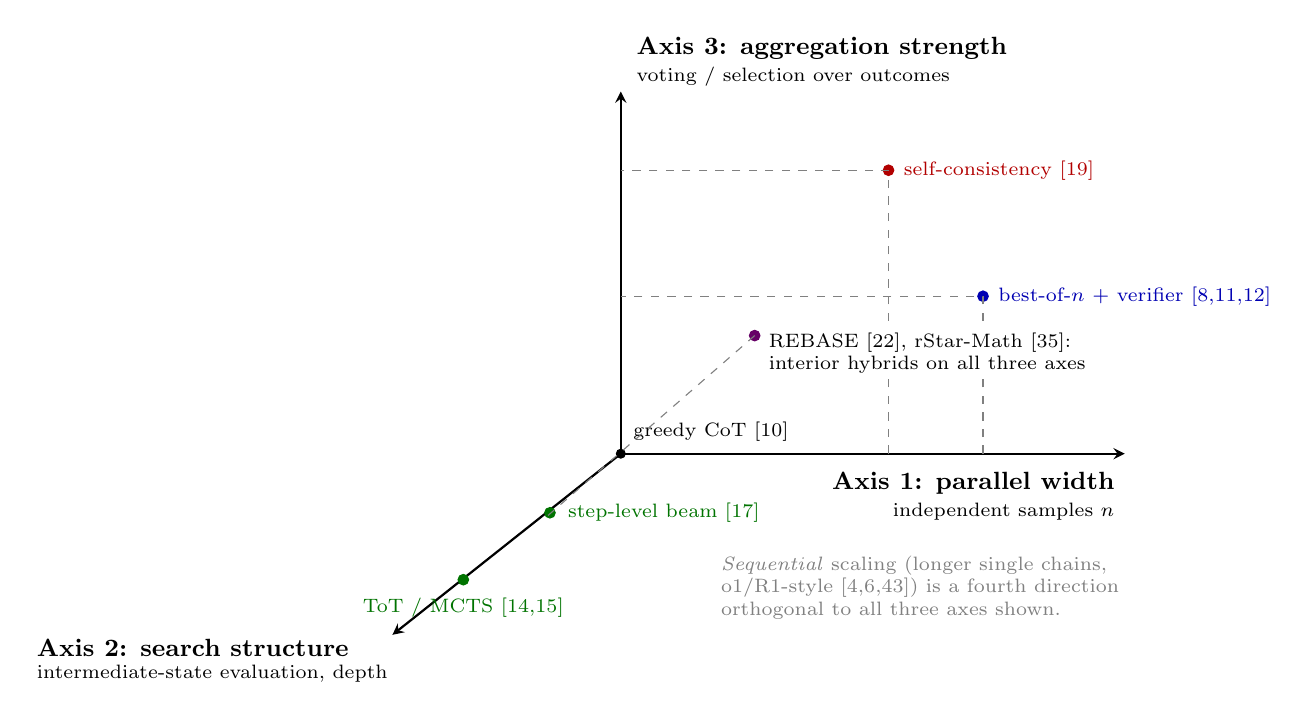
\begin{tikzpicture}[scale=1.0, >=stealth, font=\small]
% axes
\coordinate (O) at (0,0);
\draw[->, thick] (O) -- (6.4,0) node[below=3pt, anchor=north east] {\shortstack[r]{\textbf{Axis 1: parallel width}\\ \scriptsize independent samples $n$}};
\draw[->, thick] (O) -- (0,4.6) node[above left=-2pt, anchor=south west] {\shortstack[l]{\textbf{Axis 3: aggregation strength}\\ \scriptsize voting / selection over outcomes}};
\draw[->, thick] (O) -- (-2.9,-2.3) node[below left=-2pt] {\shortstack[l]{\textbf{Axis 2: search structure}\\ \scriptsize intermediate-state evaluation, depth}};
% origin point
\filldraw[black] (O) circle (1.6pt) node[above right=1pt, font=\scriptsize] {greedy CoT [10]};
% best-of-n: along width with selection
\filldraw[blue!70!black] (4.6,2.0) circle (1.9pt) node[right=2pt, font=\scriptsize, align=left] {best-of-$n$ + verifier [8,11,12]};
\draw[dashed, gray] (4.6,0) -- (4.6,2.0) -- (0,2.0);
% self-consistency: width + high aggregation
\filldraw[red!70!black] (3.4,3.6) circle (1.9pt) node[right=2pt, font=\scriptsize] {self-consistency [19]};
\draw[dashed, gray] (3.4,0) -- (3.4,3.6) -- (0,3.6);
% ToT / MCTS: structure axis
\filldraw[green!45!black] (-2.0,-1.6) circle (1.9pt) node[below=3pt, font=\scriptsize] {ToT / MCTS [14,15]};
% beam search: structure + mild width
\filldraw[green!45!black] (-0.9,-0.75) circle (1.9pt) node[right=3pt, font=\scriptsize] {step-level beam [17]};
% hybrids: interior
\filldraw[violet!80!black] (1.7,1.5) circle (1.9pt);
\node[right=2pt, font=\scriptsize, align=left, fill=white, inner sep=1.5pt] at (1.75,1.28) {REBASE [22], rStar-Math [35]:\\ interior hybrids on all three axes};
\draw[dashed, gray] (1.7,1.5) -- (-1.0,-0.85);
% long serial CoT annotation
\node[font=\scriptsize, gray, align=left] at (3.8,-1.7) {\emph{Sequential} scaling (longer single chains,\\ o1/R1-style [4,6,43]) is a fourth direction\\ orthogonal to all three axes shown.};
\end{tikzpicture}
\caption{Conceptual three-axis framework. Inference compute can be allocated independently to parallel width (more i.i.d.\ samples), search structure (evaluation and branching over partial solutions), and aggregation strength (how outcomes are combined or selected). Canonical methods occupy edges or faces of this space; most recent high-performing methods are interior hybrids whose per-axis contributions are unreported.}
\label{fig:axes}
\end{figure}

\textbf{The axes respond to different budget currencies.} Under a token or FLOP budget, axes 1 and 3 are interchangeable up to their selector, and search must justify its overhead against them [22]. Under a latency budget with abundant parallelism, axes 1 and 3 are nearly free in time while search pays for its serial depth---an asymmetry almost never surfaced because most papers report neither latency nor parallelism assumptions (Section~\ref{sec:background}). Figure~\ref{fig:axes} depicts the resulting framework. A fourth direction---\emph{sequential} scaling via longer single chains of thought, the mechanism underlying o1-class models [4,6] and controllable through budget forcing [43]---is orthogonal to all three axes and interacts with them: reasoning models make each sample longer and more expensive, shifting the compute-optimal mix, and are themselves prone to overthinking on easy inputs [44].

\section{Open Problems}
\label{sec:open}

The synthesis above supports five specific indictments of current practice, each of which defines an open problem, followed by a proposed study design.

\textbf{(1) No unified cost metric.} The surveyed papers denominate budgets in samples [19], LLM calls [42], nodes [14], tokens, FLOPs [7,22], dollars [8], and occasionally latency---and the orderings these induce are not equivalent. Speculative decoding decouples tokens from wall-clock time [23,24]; batching decouples sample count from latency; economic analyses show dollar-optimal and FLOP-optimal choices diverge [3,8]. Consequence: no meta-analysis can currently rank methods across papers. What is needed is a reporting standard that states, for every result, generated tokens, auxiliary-model tokens (verifier and value calls are compute too, and are routinely omitted), achievable parallelism, and end-to-end latency under a declared serving assumption.

\textbf{(2) No controlled single-axis ablations.} Because deployed methods are hybrids (Section~\ref{sec:comparison}), the literature contains almost no experiments that vary one axis while pinning the others. Wu et al.\ hold FLOPs fixed across whole strategies [22]; Snell et al.\ compare search against best-of-$N$ but simultaneously vary the allocation policy [7]; Liu et al.\ vary policy and reward models jointly [34]. The marginal utility of, for example, adding tree depth at fixed sample width and fixed aggregation is, at the time of writing, an unmeasured quantity in the public literature.

\textbf{(3) Verifier quality is an unisolated confound.} Axis-1 and axis-2 results are conditional on a scorer whose quality is rarely characterized independently. The evidence that this matters is direct: PRMs beat ORMs and voting with widening margins in $N$ [12]; progress-based process rewards outperform correctness-based ones [40]; Monte-Carlo step labels inject systematic noise [29,39]; imperfect verifiers convert additional samples into additional false positives [31]; proxy-reward optimization degrades gold quality [30]. A method labeled ``search beats sampling'' may in fact demonstrate ``this PRM beats that ORM.'' Open problem: benchmark inference strategies across a controlled ladder of verifier quality, from oracle checkers through strong and deliberately weakened PRMs to no verifier, so that strategy effects and scorer effects can be separated.

\textbf{(4) No predictive task taxonomy.} The synthesis shows stable task affinities---exactly verifiable tasks favor axis 1 [8], decomposable planning tasks favor axis 2 [14,22], concentrated-answer tasks favor axis 3 [19,42], and GPQA-style tasks reward none of them much [4]---but these are post-hoc observations, not predictions. No published taxonomy maps measurable task properties (answer-space entropy, verification asymmetry, step decomposability, modal-answer correctness) to the axis with the best expected marginal utility. Constructing one is a prerequisite for principled compute routing of the kind Snell et al.\ began for difficulty alone [7].

\textbf{(5) Saturation thresholds are never compared on a common basis.} Voting saturates beyond roughly $10^2$ samples [8]; best-of-$n$ saturates or reverses where verifier false positives dominate [30,31]; search saturates when the value model's discrimination is exhausted [22,40]; sequential chains saturate in overthinking [44]. Each threshold is reported in its paper's own units on its own tasks. Whether these are the same phenomenon at different scales, or genuinely different decay laws, is unknown---and it is exactly the quantity a practitioner allocating a fixed budget needs.

\textbf{Proposed follow-on study.} These gaps admit a single factorial design. Fix a small set of open-weight policy models (e.g., 1B--70B). Define a three-dimensional strategy grid: parallel width $n \in \{1,4,16,64,256\}$; search structure in \{none, beam, REBASE-style, MCTS\} at controlled node budgets; aggregation in \{none, plurality vote, verifier-weighted vote, best-of-$n$ selection\}. Cross this grid with a verifier ladder: oracle checker, strong public PRM, the same PRM degraded by label noise at known rates, and none. Evaluate on a task battery stratified ex ante by the properties in problem (4): exactly verifiable code and formal proofs, competition mathematics, multiple-choice science QA, and free-form QA. Hold \emph{total generated tokens per query} (policy plus auxiliary models) fixed within every comparison cell, and report FLOPs, latency under declared parallelism, and dollar cost alongside. The primary estimand is the marginal utility curve $\partial\,\text{accuracy} / \partial \log(\text{tokens})$ per axis, per task stratum, per verifier tier, with interaction terms estimable from the factorial structure. Pre-registration of the grid and estimands would prevent the post-hoc strategy selection that problem (5) shows is endemic. The design is expensive but bounded: it is a measurement exercise on public models, not a training effort, and its output---the first cross-axis marginal-utility table under a common budget---is precisely what Table~\ref{tab:axes} cannot currently be built from published numbers.

\section{Conclusion}
\label{sec:conclusion}

This review argued that ``test-time compute'' is not one quantity but at least three: parallel width governed by coverage and selector precision, search structure governed by value-estimate quality, and aggregation governed by the concentration of the answer distribution. Synthesizing the 2023--2026 literature under this taxonomy exposed systematic incomparability---inconsistent cost units, entangled hybrids, unisolated verifier confounds, and saturation thresholds reported without a common basis. The taxonomy's value is diagnostic: it converts a vague scaling narrative into separable mechanisms with distinct failure modes, and it makes visible that the field's most cited curves conflate them. The open-problems agenda, and in particular the factorial marginal-utility study specified in Section~\ref{sec:open}, is the necessary next step: until one axis can be varied while the others are held fixed under a shared budget, claims that any inference strategy ``scales better'' remain unfalsifiable in general form.

\section*{References}
\small\sloppy
References follow IEEE numeric style.

\begin{enumerate}
\itemsep0.15em
\item[{[1]}] J. Kaplan et al., ``Scaling laws for neural language models,'' arXiv preprint arXiv:2001.08361, 2020.
\item[{[2]}] J. Hoffmann et al., ``Training compute-optimal large language models,'' in \emph{Proc. NeurIPS}, 2022. arXiv:2203.15556.
\item[{[3]}] N. Sardana, J. Portes, S. Doubov, and J. Frankle, ``Beyond Chinchilla-optimal: Accounting for inference in language model scaling laws,'' in \emph{Proc. ICML}, 2024. arXiv:2401.00448.
\item[{[4]}] OpenAI, ``Learning to reason with LLMs,'' OpenAI Blog, Sep. 2024. [Online]. Available: \url{https://openai.com/index/learning-to-reason-with-llms/}
\item[{[5]}] A. Jaech et al., ``OpenAI o1 system card,'' arXiv preprint arXiv:2412.16720, 2024.
\item[{[6]}] DeepSeek-AI (D. Guo et al.), ``DeepSeek-R1: Incentivizing reasoning capability in LLMs via reinforcement learning,'' arXiv preprint arXiv:2501.12948, 2025.
\item[{[7]}] C. Snell, J. Lee, K. Xu, and A. Kumar, ``Scaling LLM test-time compute optimally can be more effective than scaling model parameters,'' in \emph{Proc. ICLR}, 2025. arXiv:2408.03314.
\item[{[8]}] B. Brown et al., ``Large language monkeys: Scaling inference compute with repeated sampling,'' arXiv preprint arXiv:2407.21787, 2024.
\item[{[9]}] S. Welleck et al., ``From decoding to meta-generation: Inference-time algorithms for large language models,'' \emph{Trans. Mach. Learn. Res.}, 2024. arXiv:2406.16838.
\item[{[10]}] J. Wei et al., ``Chain-of-thought prompting elicits reasoning in large language models,'' in \emph{Proc. NeurIPS}, 2022. arXiv:2201.11903.
\item[{[11]}] K. Cobbe et al., ``Training verifiers to solve math word problems,'' arXiv preprint arXiv:2110.14168, 2021.
\item[{[12]}] H. Lightman et al., ``Let's verify step by step,'' in \emph{Proc. ICLR}, 2024. arXiv:2305.20050.
\item[{[13]}] M. Chen et al., ``Evaluating large language models trained on code,'' arXiv preprint arXiv:2107.03374, 2021.
\item[{[14]}] S. Yao et al., ``Tree of thoughts: Deliberate problem solving with large language models,'' in \emph{Proc. NeurIPS}, 2023. arXiv:2305.10601.
\item[{[15]}] S. Hao et al., ``Reasoning with language model is planning with world model,'' in \emph{Proc. EMNLP}, 2023. arXiv:2305.14992.
\item[{[16]}] X. Feng et al., ``Alphazero-like tree-search can guide large language model decoding and training,'' in \emph{Proc. ICML}, 2024. arXiv:2309.17179.
\item[{[17]}] Y. Xie et al., ``Self-evaluation guided beam search for reasoning,'' in \emph{Proc. NeurIPS}, 2023. arXiv:2305.00633.
\item[{[18]}] M. Besta et al., ``Graph of thoughts: Solving elaborate problems with large language models,'' in \emph{Proc. AAAI}, 2024. arXiv:2308.09687.
\item[{[19]}] X. Wang et al., ``Self-consistency improves chain of thought reasoning in language models,'' in \emph{Proc. ICLR}, 2023. arXiv:2203.11171.
\item[{[20]}] X. Chen, R. Aksitov, U. Alon, J. Ren, K. Xiao, P. Yin, S. Prakash, C. Sutton, X. Wang, and D. Zhou, ``Universal self-consistency for large language model generation,'' arXiv preprint arXiv:2311.17311, 2023.
\item[{[21]}] Y. Li et al., ``Making language models better reasoners with step-aware verifier,'' in \emph{Proc. ACL}, 2023. arXiv:2206.02336.
\item[{[22]}] Y. Wu, Z. Sun, S. Li, S. Welleck, and Y. Yang, ``Inference scaling laws: An empirical analysis of compute-optimal inference for LLM problem-solving,'' in \emph{Proc. ICLR}, 2025. arXiv:2408.00724.
\item[{[23]}] Y. Leviathan, M. Kalman, and Y. Matias, ``Fast inference from transformers via speculative decoding,'' in \emph{Proc. ICML}, 2023. arXiv:2211.17192.
\item[{[24]}] C. Chen, S. Borgeaud, G. Irving, J.-B. Lespiau, L. Sifre, and J. Jumper, ``Accelerating large language model decoding with speculative sampling,'' arXiv preprint arXiv:2302.01318, 2023.
\item[{[25]}] N. Stiennon et al., ``Learning to summarize from human feedback,'' in \emph{Proc. NeurIPS}, 2020. arXiv:2009.01325.
\item[{[26]}] R. Nakano et al., ``WebGPT: Browser-assisted question-answering with human feedback,'' arXiv preprint arXiv:2112.09332, 2021.
\item[{[27]}] A. Beirami et al., ``Theoretical guarantees on the best-of-n alignment policy,'' arXiv preprint arXiv:2401.01879, 2024.
\item[{[28]}] J. Uesato et al., ``Solving math word problems with process- and outcome-based feedback,'' arXiv preprint arXiv:2211.14275, 2022.
\item[{[29]}] P. Wang et al., ``Math-Shepherd: Verify and reinforce LLMs step-by-step without human annotations,'' in \emph{Proc. ACL}, 2024. arXiv:2312.08935.
\item[{[30]}] L. Gao, J. Schulman, and J. Hilton, ``Scaling laws for reward model overoptimization,'' in \emph{Proc. ICML}, 2023. arXiv:2210.10760.
\item[{[31]}] B. Stroebl, S. Kapoor, and A. Narayanan, ``Inference scaling flaws: The limits of LLM resampling with imperfect verifiers,'' arXiv preprint arXiv:2411.17501, 2024.
\item[{[32]}] J. Liu, A. Cohen, R. Pasunuru, Y. Choi, H. Hajishirzi, and A. Celikyilmaz, ``Don't throw away your value model! Generating more preferable text with value-guided Monte-Carlo tree search decoding,'' in \emph{Proc. COLM}, 2024. arXiv:2309.15028.
\item[{[33]}] A. Zhou, K. Yan, M. Shlapentokh-Rothman, H. Wang, and Y.-X. Wang, ``Language agent tree search unifies reasoning, acting, and planning in language models,'' in \emph{Proc. ICML}, 2024. arXiv:2310.04406.
\item[{[34]}] R. Liu et al., ``Can 1B LLM surpass 405B LLM? Rethinking compute-optimal test-time scaling,'' arXiv preprint arXiv:2502.06703, 2025.
\item[{[35]}] X. Guan, L. L. Zhang, Y. Liu, N. Shang, Y. Sun, Y. Zhu, F. Yang, and M. Yang, ``rStar-Math: Small LLMs can master math reasoning with self-evolved deep thinking,'' arXiv preprint arXiv:2501.04519, 2025.
\item[{[36]}] Y. Tian et al., ``Toward self-improvement of LLMs via imagination, searching, and criticizing,'' in \emph{Proc. NeurIPS}, 2024. arXiv:2404.12253.
\item[{[37]}] D. Zhang, S. Zhoubian, Z. Hu, Y. Yue, Y. Dong, and J. Tang, ``ReST-MCTS*: LLM self-training via process reward guided tree search,'' in \emph{Proc. NeurIPS}, 2024. arXiv:2406.03816.
\item[{[38]}] Z. Qi et al., ``Mutual reasoning makes smaller LLMs stronger problem-solvers,'' arXiv preprint arXiv:2408.06195, 2024.
\item[{[39]}] Z. Zhang et al., ``The lessons of developing process reward models in mathematical reasoning,'' arXiv preprint arXiv:2501.07301, 2025.
\item[{[40]}] A. Setlur, C. Nagpal, A. Fisch, X. Geng, J. Eisenstein, R. Agarwal, A. Agarwal, J. Berant, and A. Kumar, ``Rewarding progress: Scaling automated process verifiers for LLM reasoning,'' in \emph{Proc. ICLR}, 2025. arXiv:2410.08146.
\item[{[41]}] P. Aggarwal, A. Madaan, Y. Yang, and Mausam, ``Let's sample step by step: Adaptive-consistency for efficient reasoning and coding with LLMs,'' in \emph{Proc. EMNLP}, 2023. arXiv:2305.11860.
\item[{[42]}] L. Chen, J. Q. Davis, B. Hanin, P. Bailis, I. Stoica, M. Zaharia, and J. Zou, ``Are more LLM calls all you need? Towards scaling laws of compound inference systems,'' in \emph{Proc. NeurIPS}, 2024. arXiv:2403.02419.
\item[{[43]}] N. Muennighoff et al., ``s1: Simple test-time scaling,'' arXiv preprint arXiv:2501.19393, 2025.
\item[{[44]}] X. Chen et al., ``Do NOT think that much for 2+3=? On the overthinking of o1-like LLMs,'' arXiv preprint arXiv:2412.21187, 2024.
\item[{[45]}] G. Luo et al., ``Improve mathematical reasoning in language models by automated process supervision,'' arXiv preprint arXiv:2406.06592, 2024.
\end{enumerate}

\end{document}
